\documentclass[serif, handout]{beamer}
\usepackage{amsmath, amssymb,amsthm}
\usepackage{tikz}

\begin{document}
\begin{figure}[h!]
\centering
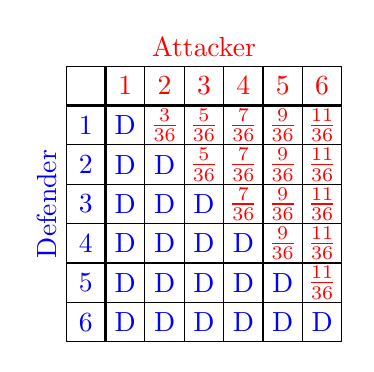
\begin{tikzpicture}[scale = 0.5, yscale = -1]
\draw (0,0) grid (7,7);
\draw[very thick] (1,0) -- (1,7) (0,1) -- (7,1);
\begin{scope}[xshift = 0.5cm, yshift = 0.5cm]
\node[red] at (3,-1) {Attacker};
\node[blue, rotate = 90] at (-1,3) {Defender};
\foreach \x in {1,2,3,4,5,6}
{
\node[red] at (\x, 0) {$\x$};
\node[blue] at (0, \x) {$\x$};
}
\foreach \attack / \p in {1/1,2/3,3/5,4/7,5/9,6/11}
{
	\foreach \defend in {1,2,3,4,5,6}
	{
		\ifnum\attack > \defend
			\node[red] at (\attack, \defend) {$\frac{\p}{36}$};
		\else
			\node[blue] at (\attack, \defend) {D};
		\fi 
	}
}
\end{scope}
\end{tikzpicture}
\end{figure}
\end{document}